\documentclass[]{article}
\usepackage{lmodern}
\usepackage{amssymb,amsmath}
\usepackage{ifxetex,ifluatex}
\usepackage{fixltx2e} % provides \textsubscript
\ifnum 0\ifxetex 1\fi\ifluatex 1\fi=0 % if pdftex
  \usepackage[T1]{fontenc}
  \usepackage[utf8]{inputenc}
\else % if luatex or xelatex
  \ifxetex
    \usepackage{mathspec}
  \else
    \usepackage{fontspec}
  \fi
  \defaultfontfeatures{Ligatures=TeX,Scale=MatchLowercase}
\fi
% use upquote if available, for straight quotes in verbatim environments
\IfFileExists{upquote.sty}{\usepackage{upquote}}{}
% use microtype if available
\IfFileExists{microtype.sty}{%
\usepackage{microtype}
\UseMicrotypeSet[protrusion]{basicmath} % disable protrusion for tt fonts
}{}
\usepackage[margin=1in]{geometry}
\usepackage{hyperref}
\hypersetup{unicode=true,
            pdftitle={Assignment 1},
            pdfauthor={Holly Finertie (HF2379)},
            pdfborder={0 0 0},
            breaklinks=true}
\urlstyle{same}  % don't use monospace font for urls
\usepackage{color}
\usepackage{fancyvrb}
\newcommand{\VerbBar}{|}
\newcommand{\VERB}{\Verb[commandchars=\\\{\}]}
\DefineVerbatimEnvironment{Highlighting}{Verbatim}{commandchars=\\\{\}}
% Add ',fontsize=\small' for more characters per line
\usepackage{framed}
\definecolor{shadecolor}{RGB}{248,248,248}
\newenvironment{Shaded}{\begin{snugshade}}{\end{snugshade}}
\newcommand{\AlertTok}[1]{\textcolor[rgb]{0.94,0.16,0.16}{#1}}
\newcommand{\AnnotationTok}[1]{\textcolor[rgb]{0.56,0.35,0.01}{\textbf{\textit{#1}}}}
\newcommand{\AttributeTok}[1]{\textcolor[rgb]{0.77,0.63,0.00}{#1}}
\newcommand{\BaseNTok}[1]{\textcolor[rgb]{0.00,0.00,0.81}{#1}}
\newcommand{\BuiltInTok}[1]{#1}
\newcommand{\CharTok}[1]{\textcolor[rgb]{0.31,0.60,0.02}{#1}}
\newcommand{\CommentTok}[1]{\textcolor[rgb]{0.56,0.35,0.01}{\textit{#1}}}
\newcommand{\CommentVarTok}[1]{\textcolor[rgb]{0.56,0.35,0.01}{\textbf{\textit{#1}}}}
\newcommand{\ConstantTok}[1]{\textcolor[rgb]{0.00,0.00,0.00}{#1}}
\newcommand{\ControlFlowTok}[1]{\textcolor[rgb]{0.13,0.29,0.53}{\textbf{#1}}}
\newcommand{\DataTypeTok}[1]{\textcolor[rgb]{0.13,0.29,0.53}{#1}}
\newcommand{\DecValTok}[1]{\textcolor[rgb]{0.00,0.00,0.81}{#1}}
\newcommand{\DocumentationTok}[1]{\textcolor[rgb]{0.56,0.35,0.01}{\textbf{\textit{#1}}}}
\newcommand{\ErrorTok}[1]{\textcolor[rgb]{0.64,0.00,0.00}{\textbf{#1}}}
\newcommand{\ExtensionTok}[1]{#1}
\newcommand{\FloatTok}[1]{\textcolor[rgb]{0.00,0.00,0.81}{#1}}
\newcommand{\FunctionTok}[1]{\textcolor[rgb]{0.00,0.00,0.00}{#1}}
\newcommand{\ImportTok}[1]{#1}
\newcommand{\InformationTok}[1]{\textcolor[rgb]{0.56,0.35,0.01}{\textbf{\textit{#1}}}}
\newcommand{\KeywordTok}[1]{\textcolor[rgb]{0.13,0.29,0.53}{\textbf{#1}}}
\newcommand{\NormalTok}[1]{#1}
\newcommand{\OperatorTok}[1]{\textcolor[rgb]{0.81,0.36,0.00}{\textbf{#1}}}
\newcommand{\OtherTok}[1]{\textcolor[rgb]{0.56,0.35,0.01}{#1}}
\newcommand{\PreprocessorTok}[1]{\textcolor[rgb]{0.56,0.35,0.01}{\textit{#1}}}
\newcommand{\RegionMarkerTok}[1]{#1}
\newcommand{\SpecialCharTok}[1]{\textcolor[rgb]{0.00,0.00,0.00}{#1}}
\newcommand{\SpecialStringTok}[1]{\textcolor[rgb]{0.31,0.60,0.02}{#1}}
\newcommand{\StringTok}[1]{\textcolor[rgb]{0.31,0.60,0.02}{#1}}
\newcommand{\VariableTok}[1]{\textcolor[rgb]{0.00,0.00,0.00}{#1}}
\newcommand{\VerbatimStringTok}[1]{\textcolor[rgb]{0.31,0.60,0.02}{#1}}
\newcommand{\WarningTok}[1]{\textcolor[rgb]{0.56,0.35,0.01}{\textbf{\textit{#1}}}}
\usepackage{longtable,booktabs}
\usepackage{graphicx,grffile}
\makeatletter
\def\maxwidth{\ifdim\Gin@nat@width>\linewidth\linewidth\else\Gin@nat@width\fi}
\def\maxheight{\ifdim\Gin@nat@height>\textheight\textheight\else\Gin@nat@height\fi}
\makeatother
% Scale images if necessary, so that they will not overflow the page
% margins by default, and it is still possible to overwrite the defaults
% using explicit options in \includegraphics[width, height, ...]{}
\setkeys{Gin}{width=\maxwidth,height=\maxheight,keepaspectratio}
\IfFileExists{parskip.sty}{%
\usepackage{parskip}
}{% else
\setlength{\parindent}{0pt}
\setlength{\parskip}{6pt plus 2pt minus 1pt}
}
\setlength{\emergencystretch}{3em}  % prevent overfull lines
\providecommand{\tightlist}{%
  \setlength{\itemsep}{0pt}\setlength{\parskip}{0pt}}
\setcounter{secnumdepth}{0}
% Redefines (sub)paragraphs to behave more like sections
\ifx\paragraph\undefined\else
\let\oldparagraph\paragraph
\renewcommand{\paragraph}[1]{\oldparagraph{#1}\mbox{}}
\fi
\ifx\subparagraph\undefined\else
\let\oldsubparagraph\subparagraph
\renewcommand{\subparagraph}[1]{\oldsubparagraph{#1}\mbox{}}
\fi

%%% Use protect on footnotes to avoid problems with footnotes in titles
\let\rmarkdownfootnote\footnote%
\def\footnote{\protect\rmarkdownfootnote}

%%% Change title format to be more compact
\usepackage{titling}

% Create subtitle command for use in maketitle
\providecommand{\subtitle}[1]{
  \posttitle{
    \begin{center}\large#1\end{center}
    }
}

\setlength{\droptitle}{-2em}

  \title{Assignment 1}
    \pretitle{\vspace{\droptitle}\centering\huge}
  \posttitle{\par}
    \author{Holly Finertie (HF2379)}
    \preauthor{\centering\large\emph}
  \postauthor{\par}
      \predate{\centering\large\emph}
  \postdate{\par}
    \date{1/17/2020}


\begin{document}
\maketitle

\begin{Shaded}
\begin{Highlighting}[]
\KeywordTok{library}\NormalTok{(tidyverse)}
\end{Highlighting}
\end{Shaded}

\begin{verbatim}
## -- Attaching packages ---------------------------------------------- tidyverse 1.2.1 --
\end{verbatim}

\begin{verbatim}
## v ggplot2 3.2.1     v purrr   0.3.2
## v tibble  2.1.3     v dplyr   0.8.3
## v tidyr   1.0.0     v stringr 1.4.0
## v readr   1.3.1     v forcats 0.4.0
\end{verbatim}

\begin{verbatim}
## -- Conflicts ------------------------------------------------- tidyverse_conflicts() --
## x dplyr::filter() masks stats::filter()
## x dplyr::lag()    masks stats::lag()
\end{verbatim}

\begin{Shaded}
\begin{Highlighting}[]
\KeywordTok{library}\NormalTok{(ggplot2)}
\end{Highlighting}
\end{Shaded}

\hypertarget{problem-1}{%
\subsection{Problem 1:}\label{problem-1}}

Please find tables below that provide summaries (min, mean, median, IQR,
max) of the quantitative features of the dataset.

\begin{Shaded}
\begin{Highlighting}[]
\NormalTok{data =}\StringTok{ }\KeywordTok{read_csv}\NormalTok{(}\StringTok{"./data/data.csv"}\NormalTok{) }\OperatorTok\StringTok{ }
\StringTok{  }\NormalTok{janitor}\OperatorTok{::}\KeywordTok{clean_names}\NormalTok{()}
\end{Highlighting}
\end{Shaded}

\begin{verbatim}
## Parsed with column specification:
## cols(
##   Age = col_double(),
##   BMI = col_double(),
##   Glucose = col_double(),
##   Insulin = col_double(),
##   HOMA = col_double(),
##   Leptin = col_double(),
##   Adiponectin = col_double(),
##   Resistin = col_double(),
##   MCP.1 = col_double(),
##   Classification = col_double()
## )
\end{verbatim}

\begin{Shaded}
\begin{Highlighting}[]
\KeywordTok{summary}\NormalTok{(data) }
\end{Highlighting}
\end{Shaded}

\begin{verbatim}
##       age            bmi           glucose          insulin      
##  Min.   :24.0   Min.   :18.37   Min.   : 60.00   Min.   : 2.432  
##  1st Qu.:45.0   1st Qu.:22.97   1st Qu.: 85.75   1st Qu.: 4.359  
##  Median :56.0   Median :27.66   Median : 92.00   Median : 5.925  
##  Mean   :57.3   Mean   :27.58   Mean   : 97.79   Mean   :10.012  
##  3rd Qu.:71.0   3rd Qu.:31.24   3rd Qu.:102.00   3rd Qu.:11.189  
##  Max.   :89.0   Max.   :38.58   Max.   :201.00   Max.   :58.460  
##       homa             leptin        adiponectin        resistin     
##  Min.   : 0.4674   Min.   : 4.311   Min.   : 1.656   Min.   : 3.210  
##  1st Qu.: 0.9180   1st Qu.:12.314   1st Qu.: 5.474   1st Qu.: 6.882  
##  Median : 1.3809   Median :20.271   Median : 8.353   Median :10.828  
##  Mean   : 2.6950   Mean   :26.615   Mean   :10.181   Mean   :14.726  
##  3rd Qu.: 2.8578   3rd Qu.:37.378   3rd Qu.:11.816   3rd Qu.:17.755  
##  Max.   :25.0503   Max.   :90.280   Max.   :38.040   Max.   :82.100  
##      mcp_1         classification 
##  Min.   :  45.84   Min.   :1.000  
##  1st Qu.: 269.98   1st Qu.:1.000  
##  Median : 471.32   Median :2.000  
##  Mean   : 534.65   Mean   :1.552  
##  3rd Qu.: 700.09   3rd Qu.:2.000  
##  Max.   :1698.44   Max.   :2.000
\end{verbatim}

\hypertarget{problem-2}{%
\subsection{Problem 2:}\label{problem-2}}

Using code below, the continuous BMI variable was transformed into a
categorical variable (bmi\_cat) with the following BMI categories:

\begin{itemize}
\tightlist
\item
  Severely underweight: BMI \textless{} 16.5kg/m\^{}2
\item
  Underweight: 16.5 \textless{}= BMI \textless{}= 18.5 kg/m\^{}2
\item
  Normal weight: 18.5 \textless{}= BMI \textless{}=24.9 kg/m\^{}2
\item
  Overweight: 25 \textless{}= BMI \textless{}= 29.9 kg/m\^{}2
\item
  Obesity class I: 30 \textless{}= BMI \textless{}= 34.9 kg/m\^{}2
\item
  Obesity class II: 35 \textless{}= BMI \textless{}= 39.9 kg/m\^{}2
\item
  Obesity class III: BMI \textgreater{}= 40 kg/m\^{}2
\end{itemize}

\begin{Shaded}
\begin{Highlighting}[]
\NormalTok{data_bmi =}\StringTok{ }\NormalTok{data }\OperatorTok\StringTok{ }
\StringTok{  }\KeywordTok{mutate}\NormalTok{(}\DataTypeTok{bmi_cat =} \KeywordTok{case_when}\NormalTok{(}
\NormalTok{      bmi }\OperatorTok{<=}\StringTok{ }\FloatTok{16.4} \OperatorTok{~}\StringTok{ "Severely underweight"}\NormalTok{, }
\NormalTok{      bmi }\OperatorTok{>=}\StringTok{ }\FloatTok{16.5} \OperatorTok{&}\StringTok{ }\NormalTok{bmi }\OperatorTok{<=}\StringTok{ }\FloatTok{18.4} \OperatorTok{~}\StringTok{ "Underweight"}\NormalTok{,}
\NormalTok{      bmi }\OperatorTok{>=}\FloatTok{18.5} \OperatorTok{&}\StringTok{ }\NormalTok{bmi }\OperatorTok{<=}\StringTok{ }\FloatTok{24.9} \OperatorTok{~}\StringTok{ "Normal weight"}\NormalTok{,}
\NormalTok{      bmi }\OperatorTok{>=}\StringTok{ }\DecValTok{25} \OperatorTok{&}\StringTok{ }\NormalTok{bmi }\OperatorTok{<=}\StringTok{ }\FloatTok{29.9} \OperatorTok{~}\StringTok{ "Overweight"}\NormalTok{, }
\NormalTok{      bmi }\OperatorTok{>=}\StringTok{ }\DecValTok{30} \OperatorTok{&}\StringTok{ }\NormalTok{bmi }\OperatorTok{<=}\StringTok{ }\FloatTok{34.9} \OperatorTok{~}\StringTok{ "Obesity 1"}\NormalTok{, }
\NormalTok{      bmi }\OperatorTok{>=}\StringTok{ }\DecValTok{35} \OperatorTok{&}\StringTok{ }\NormalTok{bmi }\OperatorTok{<=}\StringTok{ }\FloatTok{39.9} \OperatorTok{~}\StringTok{ "Obesity 2"}\NormalTok{, }
\NormalTok{      bmi }\OperatorTok{>=}\StringTok{ }\DecValTok{40} \OperatorTok{~}\StringTok{ "Obesity 3"}
\NormalTok{    )}
\NormalTok{  )}
\end{Highlighting}
\end{Shaded}

\hypertarget{problem-3}{%
\subsection{Problem 3:}\label{problem-3}}

\begin{Shaded}
\begin{Highlighting}[]
\NormalTok{data_final =}\StringTok{ }\NormalTok{data_bmi }\OperatorTok\StringTok{ }
\StringTok{  }\KeywordTok{mutate}\NormalTok{(}
    \DataTypeTok{Arm =} \KeywordTok{recode}\NormalTok{(classification, }
      \StringTok{`}\DataTypeTok{1}\StringTok{`}\NormalTok{ =}\StringTok{ "control"}\NormalTok{, }
      \StringTok{`}\DataTypeTok{2}\StringTok{`}\NormalTok{ =}\StringTok{ "case"}\NormalTok{), }
    \DataTypeTok{outcome =} \KeywordTok{recode}\NormalTok{(Arm, }
      \StringTok{"control"}\NormalTok{ =}\StringTok{ }\DecValTok{0}\NormalTok{, }
      \StringTok{"case"}\NormalTok{ =}\StringTok{ }\DecValTok{1}\NormalTok{))}
    

\NormalTok{plot =}\StringTok{ }\NormalTok{data_final }\OperatorTok\StringTok{ }
\StringTok{  }\KeywordTok{ggplot}\NormalTok{(}\KeywordTok{aes}\NormalTok{(}\DataTypeTok{x =}\NormalTok{ bmi_cat, }\DataTypeTok{fill =}\NormalTok{ Arm)) }\OperatorTok{+}
\StringTok{  }\KeywordTok{geom_bar}\NormalTok{(}\DataTypeTok{stat =} \StringTok{"count"}\NormalTok{) }\OperatorTok{+}\StringTok{ }
\StringTok{  }\KeywordTok{xlab}\NormalTok{(}\StringTok{"BMI Category"}\NormalTok{) }\OperatorTok{+}
\StringTok{  }\KeywordTok{ylab}\NormalTok{(}\StringTok{"Count of Breast CAncer Cases and Controls"}\NormalTok{) }\OperatorTok{+}
\StringTok{  }\KeywordTok{labs}\NormalTok{(}
    \DataTypeTok{title =} \StringTok{"Proportion of Breast Cancer Cases and Controls by BMI Category"}
\NormalTok{  )}

\NormalTok{plot}
\end{Highlighting}
\end{Shaded}

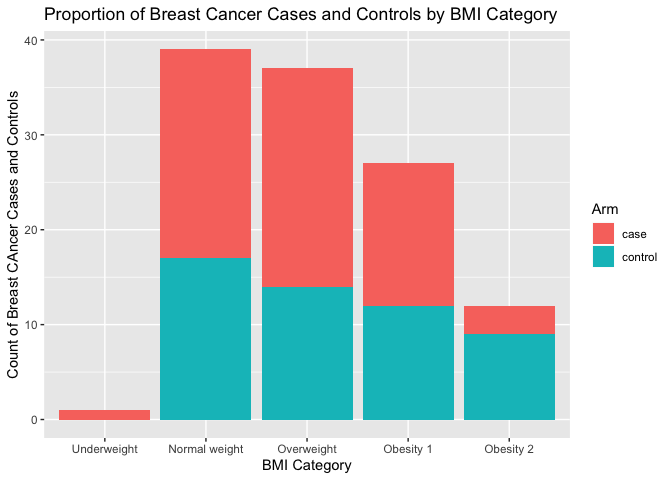
\includegraphics{pre_lecture_assignment_files/figure-latex/unnamed-chunk-4-1.pdf}

\hypertarget{problem-4}{%
\subsection{Problem 4:}\label{problem-4}}

\begin{Shaded}
\begin{Highlighting}[]
\NormalTok{logit_reg =}\StringTok{ }
\StringTok{  }\KeywordTok{glm}\NormalTok{(outcome }\OperatorTok{~}\StringTok{ }\NormalTok{glucose }\OperatorTok{+}\StringTok{ }\NormalTok{homa }\OperatorTok{+}\StringTok{ }\NormalTok{leptin }\OperatorTok{+}\StringTok{ }\NormalTok{bmi }\OperatorTok{+}\StringTok{ }\NormalTok{age, }
      \DataTypeTok{family =} \KeywordTok{binomial}\NormalTok{(}\DataTypeTok{link =} \StringTok{"logit"}\NormalTok{), }\DataTypeTok{data =}\NormalTok{ data_final) }\OperatorTok\StringTok{ }
\StringTok{  }\NormalTok{broom}\OperatorTok{::}\KeywordTok{tidy}\NormalTok{() }\OperatorTok\StringTok{ }
\StringTok{  }\KeywordTok{mutate}\NormalTok{(}
      \StringTok{"Lower Limit"}\NormalTok{ =}\StringTok{ }\NormalTok{estimate }\OperatorTok{-}\StringTok{ }\NormalTok{(std.error}\OperatorTok{*}\FloatTok{1.96}\NormalTok{), }
      \StringTok{"Upper Limit"}\NormalTok{ =}\StringTok{ }\NormalTok{estimate }\OperatorTok{+}\StringTok{ }\NormalTok{(std.error}\OperatorTok{*}\FloatTok{1.96}\NormalTok{)}
\NormalTok{  ) }\OperatorTok\StringTok{ }\KeywordTok{filter}\NormalTok{(term }\OperatorTok{==}\StringTok{ "homa"}\NormalTok{) }\OperatorTok\StringTok{ }
\StringTok{  }\KeywordTok{select}\NormalTok{(term, estimate, }\StringTok{"Lower Limit"}\NormalTok{, }\StringTok{"Upper Limit"}\NormalTok{) }\OperatorTok\StringTok{ }
\StringTok{  }\NormalTok{knitr}\OperatorTok{::}\KeywordTok{kable}\NormalTok{()}


\NormalTok{logit_reg}
\end{Highlighting}
\end{Shaded}

\begin{longtable}[]{@{}lrrr@{}}
\toprule
term & estimate & Lower Limit & Upper Limit\tabularnewline
\midrule
\endhead
homa & 0.2738822 & -0.0631907 & 0.6109551\tabularnewline
\bottomrule
\end{longtable}

As seen in the table above, the beta estimate associated with a 1-unit
change in HOMA is 0.274 with 95\% CI(-0.063, 0.611).

\hypertarget{problem-5}{%
\subsection{Problem 5:}\label{problem-5}}

\begin{Shaded}
\begin{Highlighting}[]
\NormalTok{linear_reg =}\StringTok{ }
\StringTok{  }\KeywordTok{lm}\NormalTok{(insulin }\OperatorTok{~}\StringTok{ }\NormalTok{bmi }\OperatorTok{+}\StringTok{ }\NormalTok{age }\OperatorTok{+}\StringTok{ }\NormalTok{glucose, }\DataTypeTok{data =}\NormalTok{ data_final) }\OperatorTok\StringTok{ }
\StringTok{  }\NormalTok{broom}\OperatorTok{::}\KeywordTok{tidy}\NormalTok{() }\OperatorTok\StringTok{ }
\StringTok{  }\KeywordTok{mutate}\NormalTok{(}
      \StringTok{"Lower Limit"}\NormalTok{ =}\StringTok{ }\NormalTok{estimate }\OperatorTok{-}\StringTok{ }\NormalTok{(std.error}\OperatorTok{*}\FloatTok{1.96}\NormalTok{), }
      \StringTok{"Upper Limit"}\NormalTok{ =}\StringTok{ }\NormalTok{estimate }\OperatorTok{+}\StringTok{ }\NormalTok{(std.error}\OperatorTok{*}\FloatTok{1.96}\NormalTok{)}
\NormalTok{  ) }\OperatorTok\StringTok{ }\KeywordTok{filter}\NormalTok{(term }\OperatorTok{==}\StringTok{ "age"}\NormalTok{) }\OperatorTok\StringTok{ }
\StringTok{  }\KeywordTok{select}\NormalTok{(term, estimate, }\StringTok{"Lower Limit"}\NormalTok{, }\StringTok{"Upper Limit"}\NormalTok{) }\OperatorTok\StringTok{ }
\StringTok{  }\NormalTok{knitr}\OperatorTok{::}\KeywordTok{kable}\NormalTok{()}

\NormalTok{linear_reg}
\end{Highlighting}
\end{Shaded}

\begin{longtable}[]{@{}lrrr@{}}
\toprule
term & estimate & Lower Limit & Upper Limit\tabularnewline
\midrule
\endhead
age & -0.0540217 & -0.1558221 & 0.0477787\tabularnewline
\bottomrule
\end{longtable}

As seen in the table above, the beta estimate associated with a 1-unit
change in age is -0.054 with 95\% CI(-0.156, 0.048).


\end{document}
